% Options for packages loaded elsewhere
% Options for packages loaded elsewhere
\PassOptionsToPackage{unicode}{hyperref}
\PassOptionsToPackage{hyphens}{url}
\PassOptionsToPackage{dvipsnames,svgnames,x11names}{xcolor}
%
\documentclass[
  british,
  a4paper,
]{article}
\usepackage{xcolor}
\usepackage{amsmath,amssymb}
\setcounter{secnumdepth}{-\maxdimen} % remove section numbering
\usepackage{iftex}
\ifPDFTeX
  \usepackage[T1]{fontenc}
  \usepackage[utf8]{inputenc}
  \usepackage{textcomp} % provide euro and other symbols
\else % if luatex or xetex
  \usepackage{unicode-math} % this also loads fontspec
  \defaultfontfeatures{Scale=MatchLowercase}
  \defaultfontfeatures[\rmfamily]{Ligatures=TeX,Scale=1}
\fi
\usepackage{lmodern}
\ifPDFTeX\else
  % xetex/luatex font selection
\fi
% Use upquote if available, for straight quotes in verbatim environments
\IfFileExists{upquote.sty}{\usepackage{upquote}}{}
\IfFileExists{microtype.sty}{% use microtype if available
  \usepackage[]{microtype}
  \UseMicrotypeSet[protrusion]{basicmath} % disable protrusion for tt fonts
}{}
\makeatletter
\@ifundefined{KOMAClassName}{% if non-KOMA class
  \IfFileExists{parskip.sty}{%
    \usepackage{parskip}
  }{% else
    \setlength{\parindent}{0pt}
    \setlength{\parskip}{6pt plus 2pt minus 1pt}}
}{% if KOMA class
  \KOMAoptions{parskip=half}}
\makeatother
% Make \paragraph and \subparagraph free-standing
\makeatletter
\ifx\paragraph\undefined\else
  \let\oldparagraph\paragraph
  \renewcommand{\paragraph}{
    \@ifstar
      \xxxParagraphStar
      \xxxParagraphNoStar
  }
  \newcommand{\xxxParagraphStar}[1]{\oldparagraph*{#1}\mbox{}}
  \newcommand{\xxxParagraphNoStar}[1]{\oldparagraph{#1}\mbox{}}
\fi
\ifx\subparagraph\undefined\else
  \let\oldsubparagraph\subparagraph
  \renewcommand{\subparagraph}{
    \@ifstar
      \xxxSubParagraphStar
      \xxxSubParagraphNoStar
  }
  \newcommand{\xxxSubParagraphStar}[1]{\oldsubparagraph*{#1}\mbox{}}
  \newcommand{\xxxSubParagraphNoStar}[1]{\oldsubparagraph{#1}\mbox{}}
\fi
\makeatother


\usepackage{longtable,booktabs,array}
\newcounter{none} % for unnumbered tables
\usepackage{calc} % for calculating minipage widths
% Correct order of tables after \paragraph or \subparagraph
\usepackage{etoolbox}
\makeatletter
\patchcmd\longtable{\par}{\if@noskipsec\mbox{}\fi\par}{}{}
\makeatother
% Allow footnotes in longtable head/foot
\IfFileExists{footnotehyper.sty}{\usepackage{footnotehyper}}{\usepackage{footnote}}
\makesavenoteenv{longtable}
\usepackage{graphicx}
\makeatletter
\newsavebox\pandoc@box
\newcommand*\pandocbounded[1]{% scales image to fit in text height/width
  \sbox\pandoc@box{#1}%
  \Gscale@div\@tempa{\textheight}{\dimexpr\ht\pandoc@box+\dp\pandoc@box\relax}%
  \Gscale@div\@tempb{\linewidth}{\wd\pandoc@box}%
  \ifdim\@tempb\p@<\@tempa\p@\let\@tempa\@tempb\fi% select the smaller of both
  \ifdim\@tempa\p@<\p@\scalebox{\@tempa}{\usebox\pandoc@box}%
  \else\usebox{\pandoc@box}%
  \fi%
}
% Set default figure placement to htbp
\def\fps@figure{htbp}
\makeatother



\ifLuaTeX
\usepackage[bidi=basic,shorthands=off]{babel}
\else
\usepackage[bidi=default,shorthands=off]{babel}
\fi
\ifLuaTeX
  \usepackage{selnolig} % disable illegal ligatures
\fi


\setlength{\emergencystretch}{3em} % prevent overfull lines

\providecommand{\tightlist}{%
  \setlength{\itemsep}{0pt}\setlength{\parskip}{0pt}}



 


\makeatletter
\@ifpackageloaded{tcolorbox}{}{\usepackage[skins,breakable]{tcolorbox}}
\@ifpackageloaded{fontawesome5}{}{\usepackage{fontawesome5}}
\definecolor{quarto-callout-color}{HTML}{909090}
\definecolor{quarto-callout-note-color}{HTML}{0758E5}
\definecolor{quarto-callout-important-color}{HTML}{CC1914}
\definecolor{quarto-callout-warning-color}{HTML}{EB9113}
\definecolor{quarto-callout-tip-color}{HTML}{00A047}
\definecolor{quarto-callout-caution-color}{HTML}{FC5300}
\definecolor{quarto-callout-color-frame}{HTML}{acacac}
\definecolor{quarto-callout-note-color-frame}{HTML}{4582ec}
\definecolor{quarto-callout-important-color-frame}{HTML}{d9534f}
\definecolor{quarto-callout-warning-color-frame}{HTML}{f0ad4e}
\definecolor{quarto-callout-tip-color-frame}{HTML}{02b875}
\definecolor{quarto-callout-caution-color-frame}{HTML}{fd7e14}
\makeatother
\makeatletter
\@ifpackageloaded{caption}{}{\usepackage{caption}}
\AtBeginDocument{%
\ifdefined\contentsname
  \renewcommand*\contentsname{Table of contents}
\else
  \newcommand\contentsname{Table of contents}
\fi
\ifdefined\listfigurename
  \renewcommand*\listfigurename{List of Figures}
\else
  \newcommand\listfigurename{List of Figures}
\fi
\ifdefined\listtablename
  \renewcommand*\listtablename{List of Tables}
\else
  \newcommand\listtablename{List of Tables}
\fi
\ifdefined\figurename
  \renewcommand*\figurename{Figure}
\else
  \newcommand\figurename{Figure}
\fi
\ifdefined\tablename
  \renewcommand*\tablename{Table}
\else
  \newcommand\tablename{Table}
\fi
}
\@ifpackageloaded{float}{}{\usepackage{float}}
\floatstyle{ruled}
\@ifundefined{c@chapter}{\newfloat{codelisting}{h}{lop}}{\newfloat{codelisting}{h}{lop}[chapter]}
\floatname{codelisting}{Listing}
\newcommand*\listoflistings{\listof{codelisting}{List of Listings}}
\makeatother
\makeatletter
\makeatother
\makeatletter
\@ifpackageloaded{caption}{}{\usepackage{caption}}
\@ifpackageloaded{subcaption}{}{\usepackage{subcaption}}
\makeatother
\usepackage{bookmark}
\IfFileExists{xurl.sty}{\usepackage{xurl}}{} % add URL line breaks if available
\urlstyle{same}
% fallback for those not using the hyperref driver hyperxmp:
\makeatletter
\@ifundefined{xmpquote}{\newcommand{\xmpquote}[1]{#1}}{}
\makeatother
\hypersetup{
  pdftitle={One engine{,} many forecasting methods{,} back-tested across 20 economies},
  pdfauthor={Carlos Galindo},
  pdflang={en-GB},
  colorlinks=true,
  linkcolor={blue},
  filecolor={Maroon},
  citecolor={Blue},
  urlcolor={Blue},
  pdfcreator={LaTeX via pandoc}}


\title{One engine, many forecasting methods, back-tested across 20
economies}
\usepackage{etoolbox}
\makeatletter
\providecommand{\subtitle}[1]{% add subtitle to \maketitle
  \apptocmd{\@title}{\par {\large #1 \par}}{}{}
}
\makeatother
\subtitle{An automated price-forecasting engine that fits several
methods per series, combines them, and is back-tested against a naive
benchmark}
\author{Carlos Galindo}
\date{}
\begin{document}
\maketitle


\begin{tcolorbox}[enhanced jigsaw, arc=.35mm, bottomrule=.15mm, breakable, colback=white, colframe=quarto-callout-note-color-frame, left=2mm, leftrule=.75mm, opacityback=0, rightrule=.15mm, toprule=.15mm]

\vspace{-3mm}\textbf{At a glance}\vspace{3mm}

\begin{itemize}
\tightlist
\item
  \textbf{Question.} Can one automated engine produce credible monthly
  price forecasts for many economies, and can we say rigorously whether
  it beats a simple benchmark?
\item
  \textbf{Approach.} Per series: remove seasonality, fit several
  regression-based forecasts, combine them using their track record, and
  judge the result in a rolling back-test against a naive forecast.
\item
  \textbf{Finding.} The engine was rebuilt and back-tested for price
  forecasts in 20 economies, including the UK, over 2024--2025. The
  design makes the comparison with a naive benchmark routine rather than
  an afterthought.
\item
  \textbf{Why it matters.} Forecast users need to know not just a number
  but whether the method behind it earns its complexity.
\end{itemize}

\end{tcolorbox}

\subsection{The question}\label{the-question}

Price forecasting is usually done country by country, series by series,
with a favoured model for each. That works for one economy and breaks
down when the job is to cover twenty: the favoured model differs by
place, the data arrive in different forms, and nobody can say whether a
given forecast is better than simply carrying last year's pattern
forward.

The work described here began in a previous role as a set of forecasting
routines and was rebuilt and improved during a period of independent
research. The aim was an \emph{automated multi-method engine}: give it a
monthly price series for any economy, and it returns a set of forecasts
from several different methods, a combined forecast, and a scorecard
against a naive benchmark. The point is not any single model. It is a
procedure that treats the choice of model as something to be tested,
series by series.

Two shortcomings of the obvious approach motivated this. First, a single
model's good run is easily mistaken for skill; the benchmark question
(``would doing nothing clever have done as well?'') is rarely asked.
Second, a forecast that looks excellent in a back-test can be so only
because the test quietly used information the forecaster would not have
had. A multi-country engine multiplies both risks, so the discipline has
to be built into the engine itself.

\subsection{Approach}\label{approach}

\textbf{Data.} Monthly consumer-price series, one economy at a time, in
whatever form the source supplies: an index level, a month-on-month
change, or a year-on-year rate. The engine first converts every input to
a common form, a price index, so that the same machinery can run on all
of them. Forecasts are made as month-on-month changes, chained into an
index, and reported as year-on-year rates, so the monthly and annual
views cannot disagree.

\textbf{Methods.} For each series the engine fits several forecasting
specifications and keeps all of them rather than a single winner.

\begin{itemize}
\tightlist
\item
  \emph{Naive benchmark.} A forecast built only from the series' own
  recent pattern, with no explanatory variables. It is the bar every
  other method must clear.
\item
  \emph{Regression on the series' own history.} The month-on-month
  change is regressed on seasonal indicators and on its own lags up to
  twelve months back, plus short moving averages at different lags.
  Which regressors stay is decided by stepwise selection, adding and
  dropping terms by significance, so that each series gets the
  specification its own history supports.
\item
  \emph{Robust variants.} The same regression is re-estimated in a way
  that limits the influence of outliers, with a fall-back to ordinary
  estimation if the robust fit fails, so one awkward series does not
  stop a multi-country run.
\item
  \emph{Structural-break variant.} The regression is re-fitted allowing
  for up to seven structural breaks, because inflation relationships
  shift (energy shocks, policy regimes, changes in measurement).
\item
  \emph{Seasonal-adjustment treatment.} Forecasts can be passed through
  a model-based seasonal decomposition, so that seasonal patterns that
  drift over time are not frozen at their historical average.
\end{itemize}

\textbf{Combination.} The individual forecasts are combined with weights
based on rank: methods with smaller past errors count for more. A second
combination weights by past squared error. The final forecast is an
equal blend of the two. Combining methods is a long-established way to
hedge against any single specification being wrong, and it is the one
item on this list that a reader can expect to help on average.

\textbf{Back-testing.} The engine holds the data back at a chosen date,
treats the remaining history as all that is known, and forecasts 24
months ahead. It then rolls the date forward and repeats. At each date
everything is re-estimated from the data available at that date,
including the selection of regressors. Errors are collected by horizon
and compared with the naive benchmark's errors over the same windows.
This is run for each economy in turn, and the work covered 20 economies,
including the UK, over 2024--2025.

\subsection{What the work shows}\label{what-the-work-shows}

The substantive result of the rebuild is a working, repeatable procedure
rather than a single headline number: an engine that, for any monthly
price series, produces a family of forecasts, a combined forecast, and a
benchmark comparison from a rolling back-test, across 20 economies. The
pattern of results the design is built to expose can be illustrated on
simulated series that mimic the structure (20 economies, monthly data,
horizons up to 12 months, a rolling set of forecast origins).

\begin{figure}

\centering{

\pandocbounded{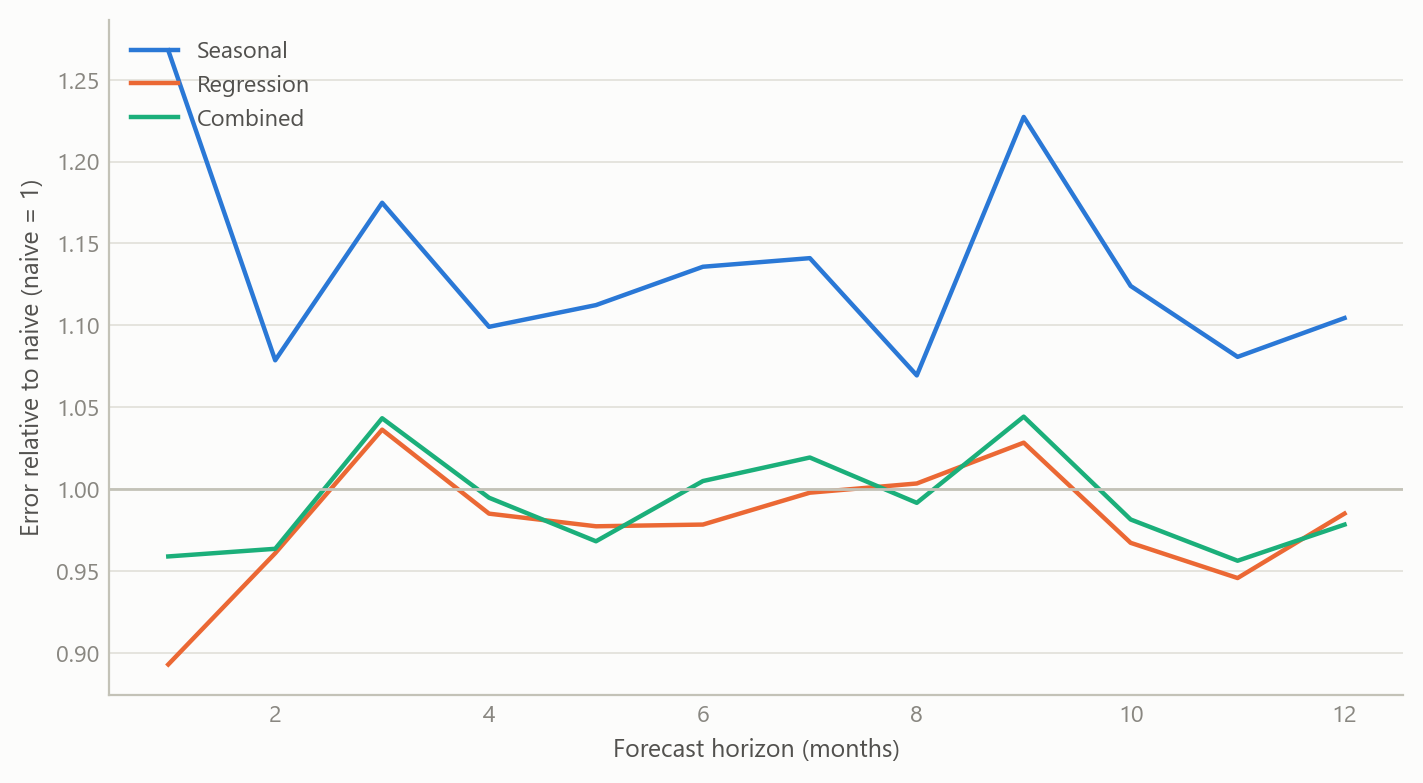
\includegraphics[keepaspectratio]{index_files/figure-latex/fig-relative-output-1.png}}

}

\caption{\label{fig-relative}Forecast error relative to the naive
benchmark, by horizon, averaged over 20 simulated economies (simulated
data). Below 1 means better than naive.}

\end{figure}%

The shape that matters is in the figure: no method need be best at every
horizon, the combination tends to track the better of its ingredients,
and a poorly specified method can lose to the naive benchmark at every
horizon. That is why the engine reports every method against the
benchmark instead of announcing a winner.

\begin{figure}

\centering{

\pandocbounded{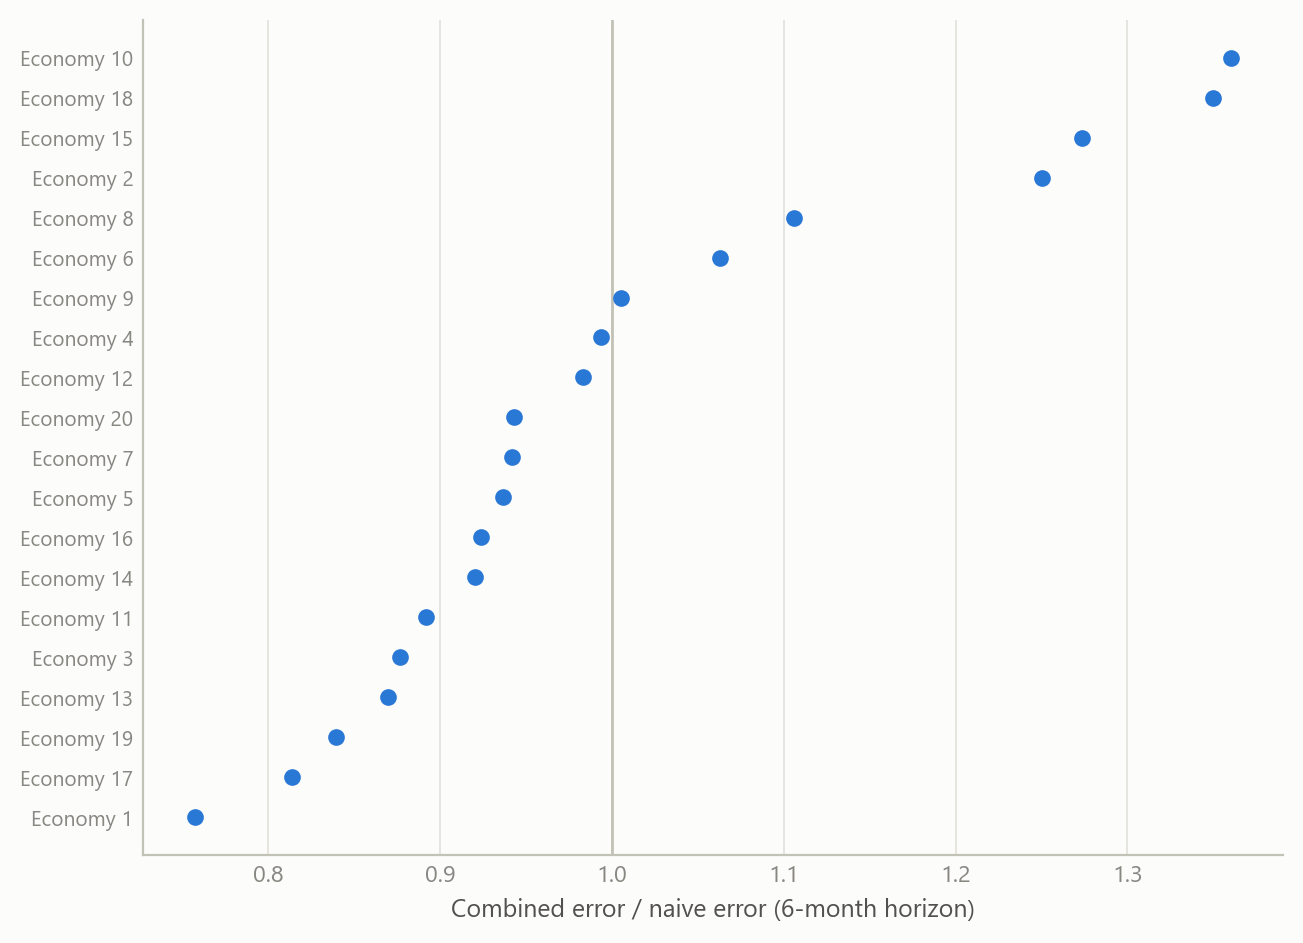
\includegraphics[keepaspectratio]{index_files/figure-latex/fig-economies-output-1.png}}

}

\caption{\label{fig-economies}Combined forecast error relative to naive
at a 6-month horizon, by simulated economy (simulated data). Dots to the
left of 1 beat the benchmark.}

\end{figure}%

Across economies the verdict is not uniform: in the simulated panel the
combined forecast beats the benchmark in most economies at this horizon
and loses in a few. A multi-country engine should therefore be judged by
the distribution of outcomes, not by its best country.

\begin{figure}

\centering{

\pandocbounded{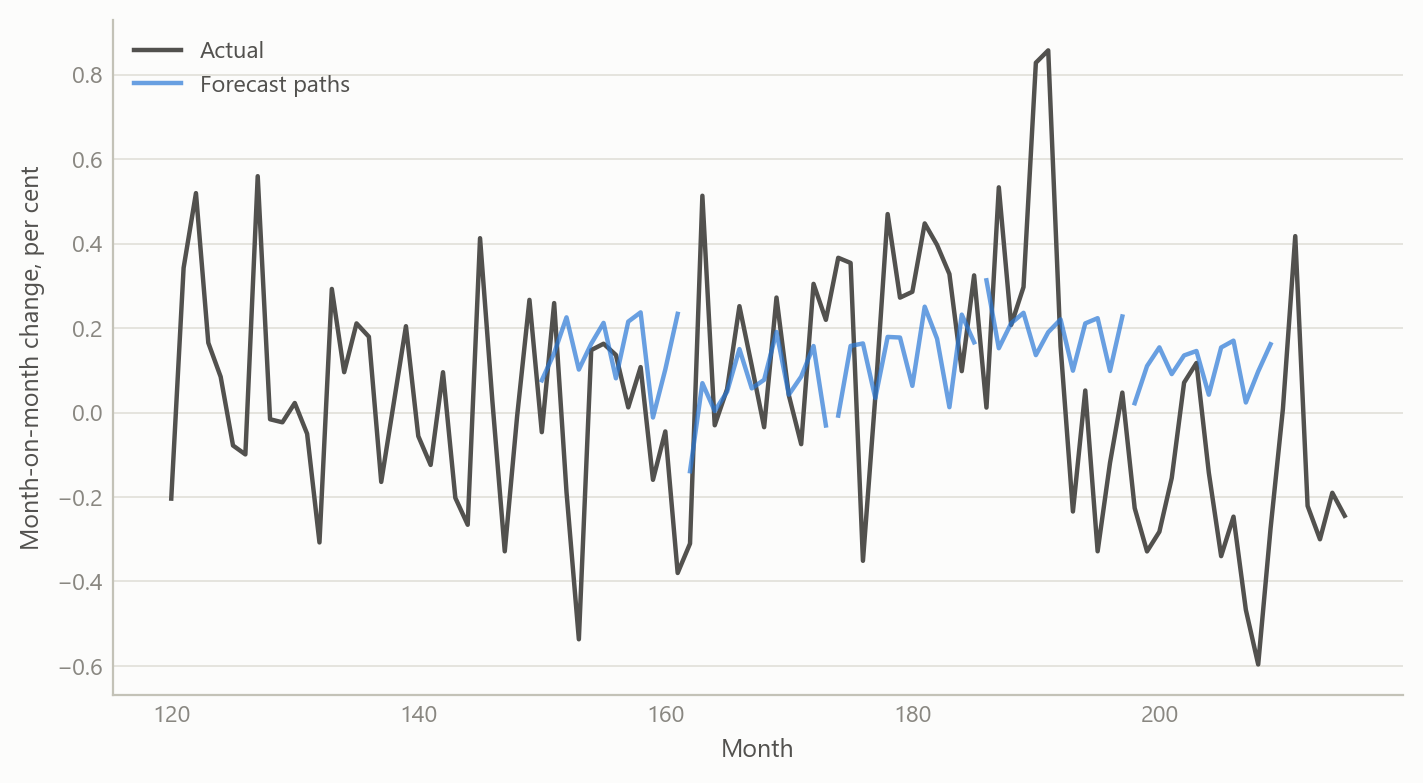
\includegraphics[keepaspectratio]{index_files/figure-latex/fig-origins-output-1.png}}

}

\caption{\label{fig-origins}One simulated economy: a rolling set of
forecast paths launched from successive origins (simulated data).}

\end{figure}%

\subsection{Insights}\label{insights}

\begin{enumerate}
\def\labelenumi{\arabic{enumi}.}
\tightlist
\item
  \textbf{Build the benchmark into the engine.} The naive forecast is
  produced for every series every time, so that ``does this beat doing
  nothing clever?'' is answered by default.
\item
  \textbf{Keep the ensemble, not a winner.} Selecting the best-looking
  model per series rewards luck. Retaining several and combining them on
  track record is a cheap hedge against specification error.
\item
  \textbf{A back-test is only as reliable as its information set.}
  Everything, including variable selection, must be redone from the data
  available at each origin. A test that lets any later information leak
  (a later benchmark forecast, a better-informed oil price path) will
  flatter the model. Reviewing the wider forecasting system later made
  this concrete: the settings that make a test clean are not always the
  defaults, and an engine should say so on its face.
\item
  \textbf{Automation needs graceful failure.} Robust estimation with a
  fall-back, and break-tolerant specifications, keep a twenty-economy
  run going when one series misbehaves.
\item
  \textbf{Judge the distribution of outcomes.} Report how many economies
  and horizons beat the benchmark, and by how much, rather than the best
  case.
\end{enumerate}

\subsection{Scope and next steps}\label{scope-and-next-steps}

The sources I salvaged document the design of the engine and the
existence of back-test runs for 2024--2025; they do not contain a
finished results table, so this note makes no claim about how large the
gains over the naive benchmark were. The figures here are simulated and
show the method's logic only.

The forecasts also depend on the quality of the underlying price data,
which differ in revisions and definitions across economies. Point
accuracy is judged here; calibrated probability bands would need a
separate evaluation. Next steps are to re-extract the stored back-test
results into a clean per-economy table, add a UK panel, and test whether
the combination weights remain stable across origins.

\subsection{About the evidence}\label{about-the-evidence}

The work is real and was done during an independent research period, May
2024 onward: a rebuilt automated engine, applied in back-tests to price
forecasts in 20 economies including the UK, in 2024--2025, and developed
with AI assistance as a systems architect. What you see on this page is
illustrative. Every figure is simulated.

Figures and tables marked \emph{simulated} are generated from simulated
data built to share the structure of the analysis (its variables,
horizons and frequencies). They show how each method works and what its
output looks like. Results stated in the text, and figures that give a
source, are the project's own. Methods are described at the level of a
methods section. Code and data pipelines are not reproduced here.




\end{document}
